\documentclass[12pt,a4paper]{article}

% ---- PACKAGES ----
\usepackage[utf8]{inputenc}
\usepackage[T1]{fontenc}
\usepackage[bahasa]{babel}
\usepackage{graphicx}
\usepackage{booktabs}
\usepackage{array}
\usepackage{geometry}
\usepackage{hyperref}
\usepackage{float}
\usepackage{caption}
\usepackage{setspace}
\usepackage{xcolor}
\usepackage{tabularx}

% ---- SETTINGS ----
\geometry{top=2.5cm, left=2.5cm, right=2.5cm, bottom=2.5cm}
\setstretch{1.15}
\hypersetup{colorlinks=true, linkcolor=black, urlcolor=blue}

\graphicspath{{./}}

\begin{document}

% ============================================================
% HALAMAN JUDUL
% ============================================================
\begin{titlepage}
\centering
\vspace*{2cm}
{\LARGE\bfseries Laporan Manipulasi Citra Digital\\[0.3cm]
Menggunakan OpenCV\par}
\vspace{1cm}
{\large Mata Kuliah: Pengolahan Sinyal Digital\par}
\vspace{2cm}
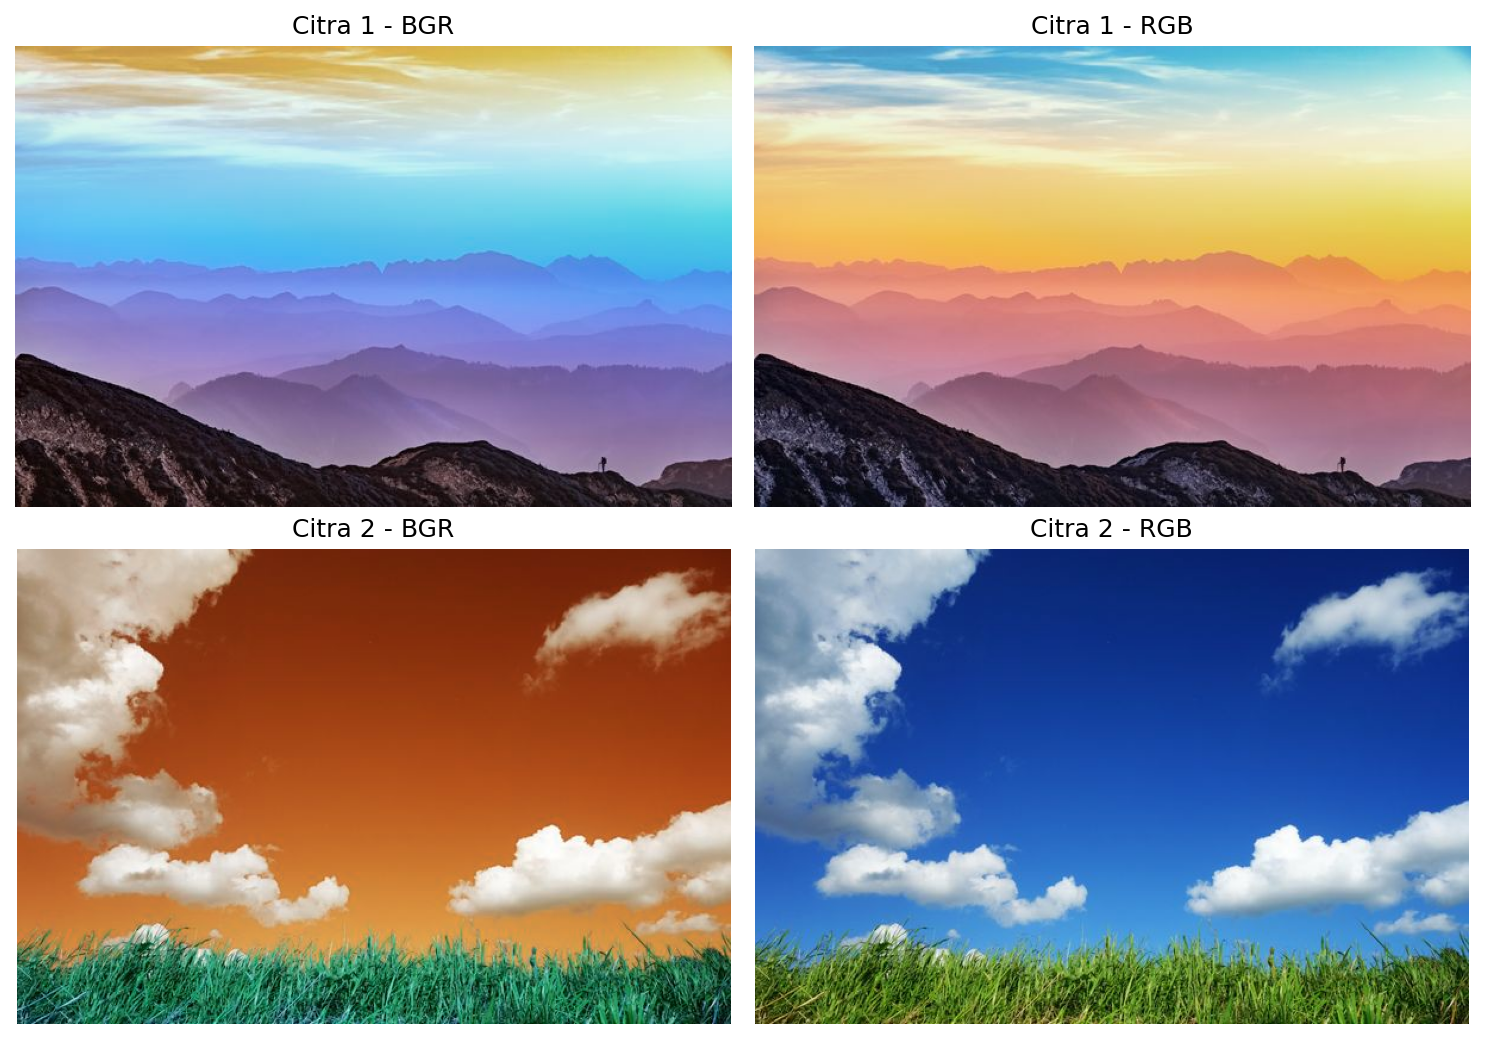
\includegraphics[width=4cm]{fig1_bgr_rgb.png}\par\vspace{0.5cm}
\vspace{2cm}

\begin{tabular}{rl}
Nama & : Farrel Ghozy Affifudin\\
NIM & : 452024611053\\
Kelas & : TI5 A2\\
Program Studi & : Teknik Informatika\\
Fakultas & : Sains dan Teknologi\\
Universitas & : Universitas Darussalam Gontor\\
\end{tabular}

\vfill
\centering
Tahun Akademik 2025/2026
\end{titlepage}

% ============================================================
% 1. PENDAHULUAN
% ============================================================
\section{Pendahuluan}

Citra digital merupakan representasi visual dari suatu objek dalam bentuk matriks nilai pixel.
Setiap pixel menyimpan informasi intensitas cahaya yang dapat dimanipulasi secara matematis
untuk menghasilkan efek visual tertentu. Tugas ini bertujuan untuk memahami bagaimana operasi
matematis sederhana dapat mengubah karakteristik visual citra digital menggunakan Python dan
OpenCV.

Eksperimen yang dilakukan meliputi: membaca dan menampilkan citra, konversi warna BGR ke RGB,
resize, image blending, image negative, transformasi logaritmik, dan transformasi gamma.
Setiap teknik dianalisis berdasarkan pengaruhnya terhadap brightness, contrast, dan detail citra.

% ============================================================
% 2. CITRA YANG DIGUNAKAN
% ============================================================
\section{Citra yang Digunakan}

Dua citra berbeda digunakan dalam eksperimen ini (Tabel~\ref{tab:citra}):

\begin{table}[H]
\centering
\caption{Spesifikasi citra yang digunakan}
\label{tab:citra}
\begin{tabular}{llll}
\toprule
\textbf{Citra} & \textbf{Sumber} & \textbf{Dimensi} & \textbf{Karakteristik}\\
\midrule
image1.jpg & Pexels.com & 600 $\times$ 386 & Terang, detail tinggi\\
image2.jpg & Pexels.com & 600 $\times$ 400 & Gelap, kontras rendah\\
\bottomrule
\end{tabular}
\end{table}

\begin{figure}[H]
\centering
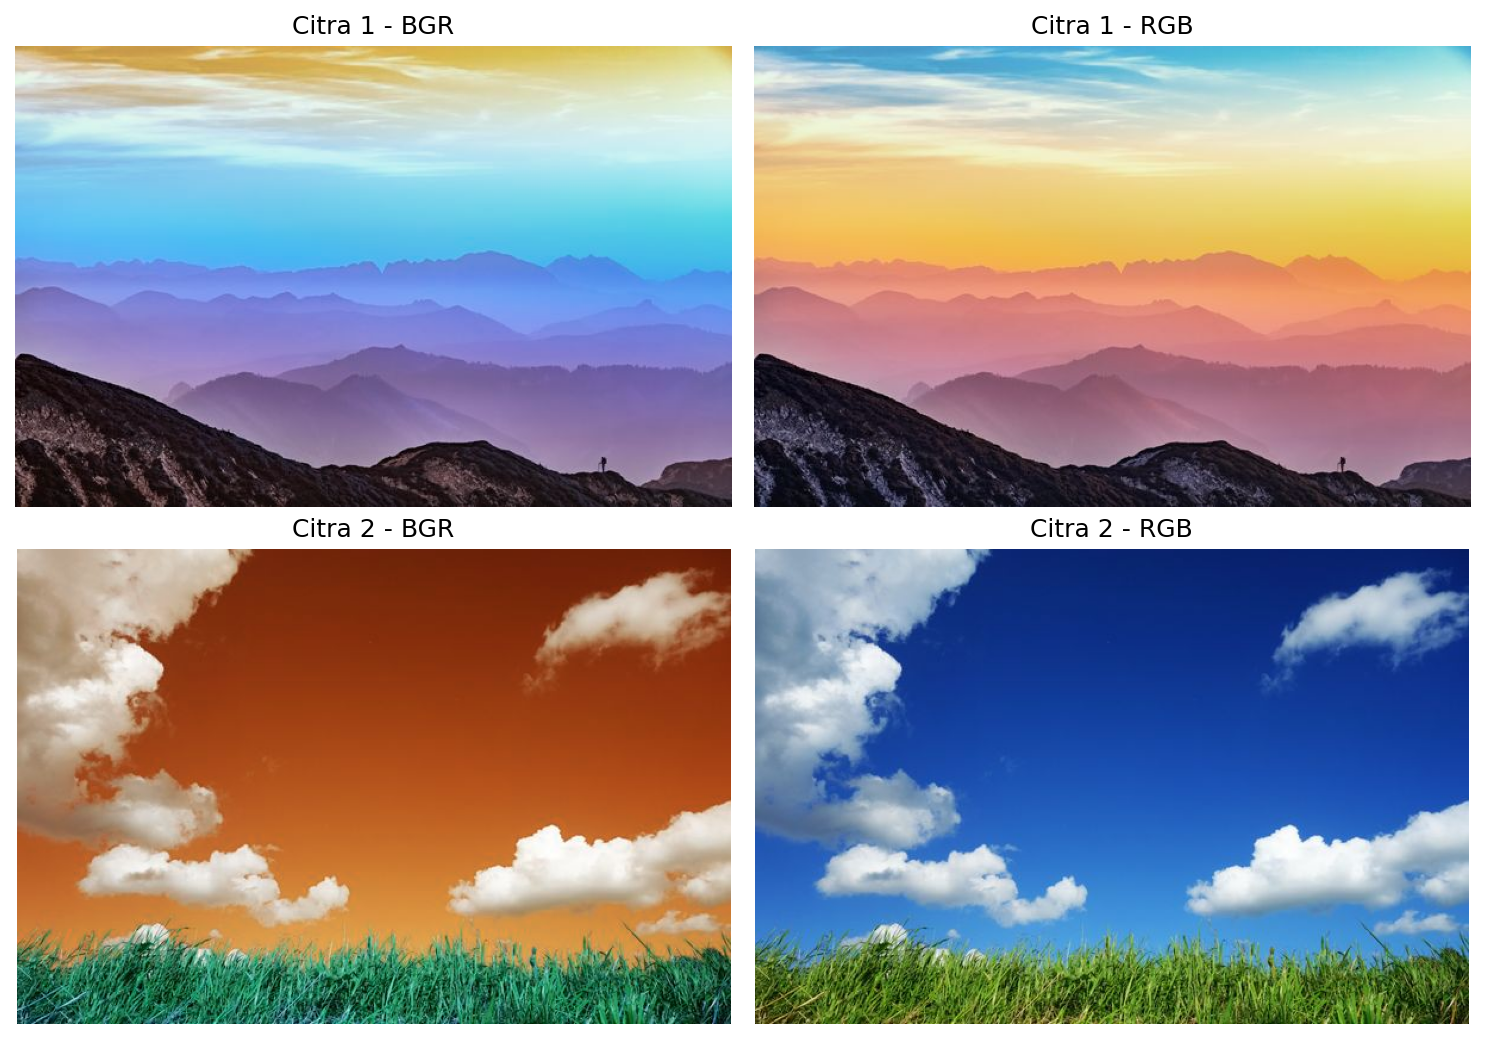
\includegraphics[width=0.9\textwidth]{fig1_bgr_rgb.png}
\caption{Perbandingan citra BGR (kiri) dan RGB (kanan)}
\label{fig:bgr_rgb}
\end{figure}

% ============================================================
% 3. MEMBACA CITRA DAN KONVERSI WARNA
% ============================================================
\section{Membaca Citra dan Konversi Warna}

\subsection{Membaca Citra}
Kedua citra dibaca menggunakan fungsi \texttt{cv2.imread()}. OpenCV membaca citra dalam format
BGR (Blue-Green-Red), bukan RGB (Red-Green-Blue). Hasil pembacaan ditampilkan pada
Tabel~\ref{tab:info_citra}.

\begin{table}[H]
\centering
\caption{Informasi citra sebelum konversi}
\label{tab:info_citra}
\begin{tabular}{lcccc}
\toprule
\textbf{Citra} & \textbf{Shape} & \textbf{Tipe Data} & \textbf{Min Pixel} & \textbf{Max Pixel}\\
\midrule
Citra 1 & (386, 600, 3) & uint8 & 0 & 255\\
Citra 2 & (400, 600, 3) & uint8 & 0 & 255\\
\bottomrule
\end{tabular}
\end{table}

\subsection{Konversi BGR ke RGB}
Konversi dilakukan dengan \texttt{cv2.cvtColor(img, cv2.COLOR\_BGR2RGB)}. Hasil konversi
ditunjukkan pada Gambar~\ref{fig:bgr_rgb}. Warna pada citra BGR tampak tidak natural karena
channel merah dan biru tertukar saat ditampilkan dengan Matplotlib yang menggunakan format RGB.

\subsection{Jawaban Analisis}

\textbf{1. Mengapa warna citra tidak sesuai jika langsung ditampilkan setelah dibaca OpenCV?}
OpenCV membaca citra dalam format BGR, sedangkan Matplotlib menggunakan RGB. Akibatnya,
channel biru dan merah tertukar sehingga warna tampak aneh.

\textbf{2. Apa perbedaan BGR dan RGB?}
BGR dan RGB adalah format urutan channel warna. RGB: Red--Green--Blue (Matplotlib, monitor).
BGR: Blue--Green--Red (OpenCV secara default).

\textbf{3. Mengapa penting memahami format warna?}
Agar manipulasi channel warna dilakukan pada channel yang benar, mencegah kesalahan pemrosesan.

% ============================================================
% 4. IMAGE BLENDING
% ============================================================
\section{Image Blending}

Image blending menggabungkan dua citra menggunakan persamaan $I_{blend} = \alpha I_1 + \beta I_2 + \gamma$
dengan syarat $\alpha + \beta = 1$. Kedua citra di-resize terlebih dahulu ke ukuran 600 $\times$ 400.

\begin{table}[H]
\centering
\caption{Hasil image blending dengan variasi bobot}
\label{tab:blending}
\begin{tabular}{ccc}
\toprule
$\alpha$ & $\beta$ & Analisis Hasil\\
\midrule
0,2 & 0,8 & Citra 2 (gelap) lebih dominan, hasil cenderung gelap\\
0,5 & 0,5 & Kedua citra seimbang, detail dari keduanya terlihat\\
0,8 & 0,2 & Citra 1 (terang) lebih dominan, hasil cenderung terang\\
\bottomrule
\end{tabular}
\end{table}

\begin{figure}[H]
\centering
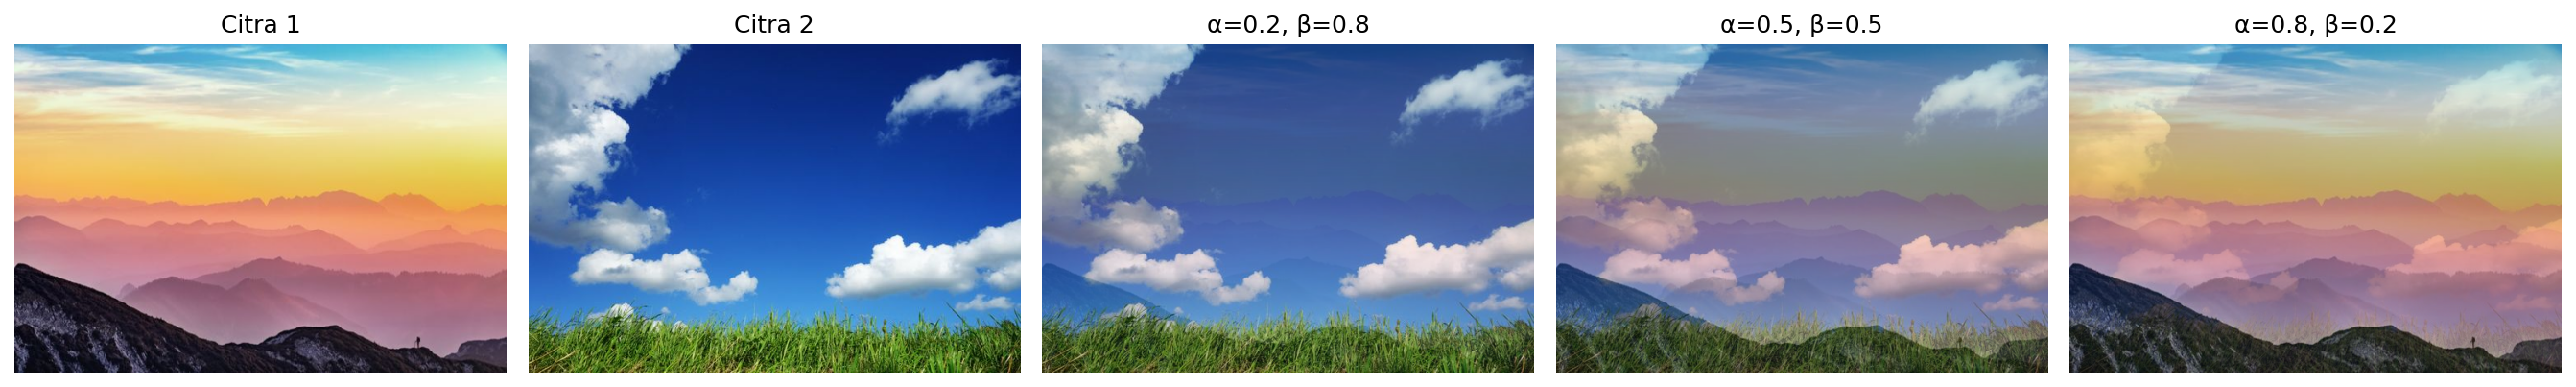
\includegraphics[width=\textwidth]{fig2_blending.png}
\caption{Hasil image blending dengan tiga kombinasi bobot}
\label{fig:blending}
\end{figure}

\textbf{Jawaban Analisis:}
\begin{enumerate}
\item Semakin besar $\alpha$, citra pertama semakin dominan. Semakin besar $\beta$, citra kedua dominan.
\item Jika $\alpha + \beta > 1$, nilai pixel dapat melebihi 255 (saturasi/clipping).
\item Aplikasi nyata: watermarking, efek transisi, augmented reality, komposisi foto.
\end{enumerate}

% ============================================================
% 5. IMAGE NEGATIVE
% ============================================================
\section{Image Negative}

Operasi image negative menggunakan persamaan $I_{negatif} = 255 - I$. Hasilnya, pixel terang
menjadi gelap dan sebaliknya.

\begin{figure}[H]
\centering
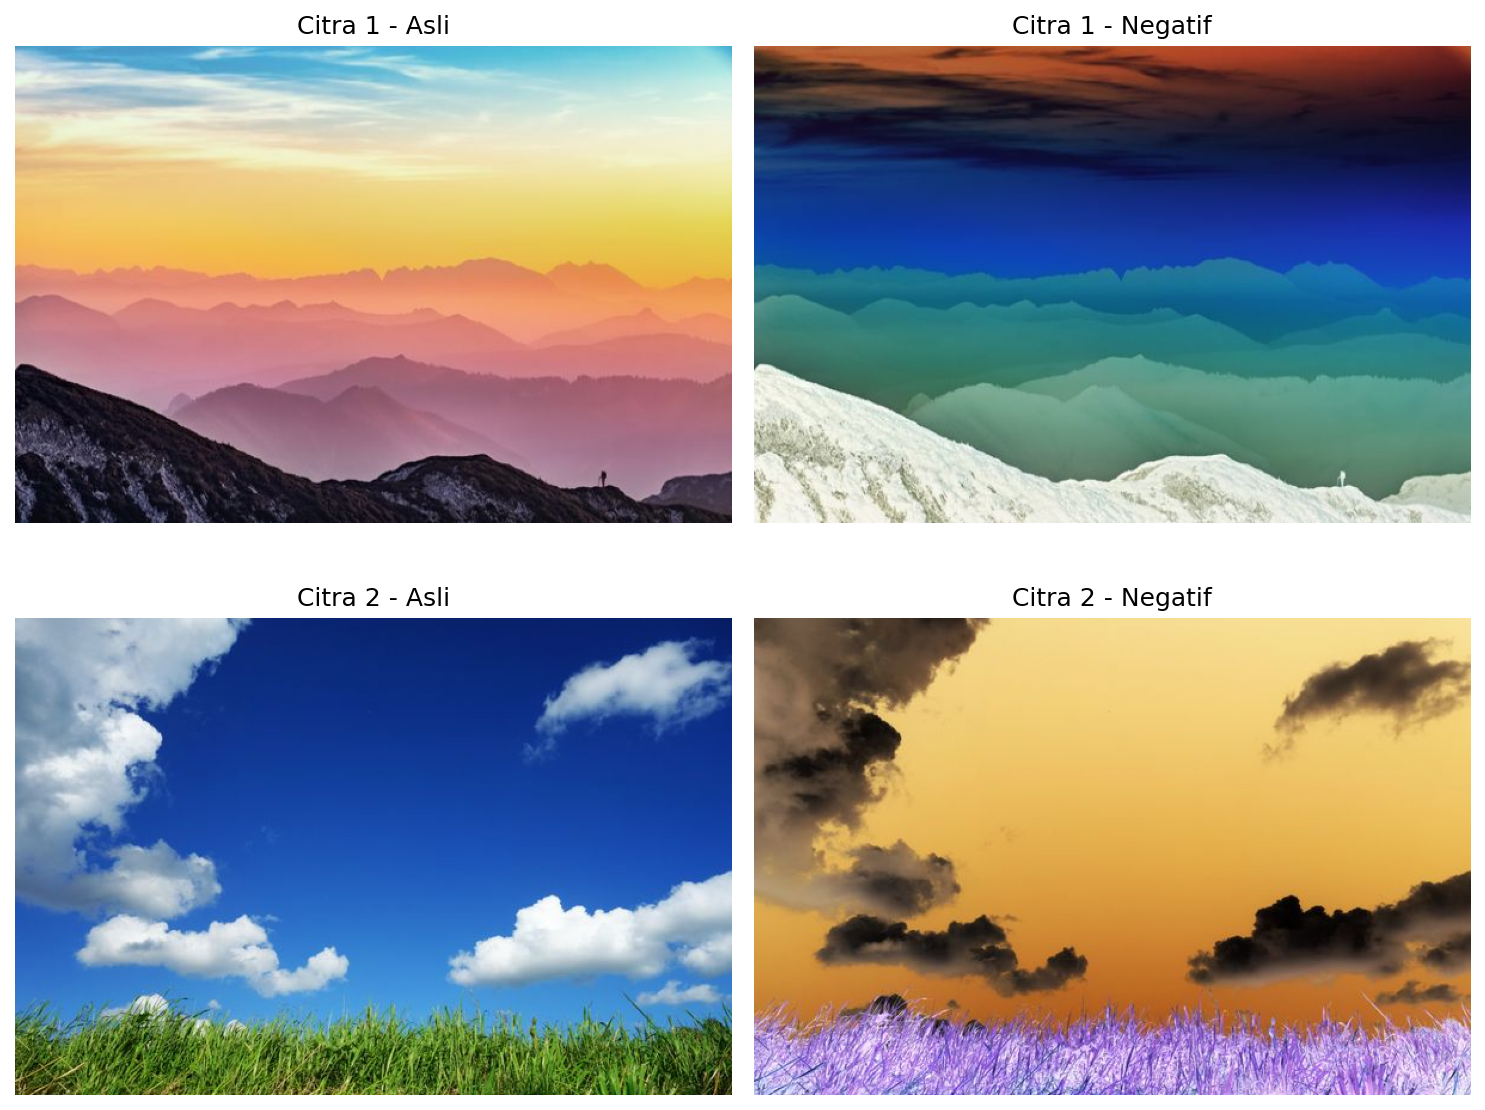
\includegraphics[width=0.85\textwidth]{fig3_negative.png}
\caption{Perbandingan citra asli dan citra negatif}
\label{fig:negative}
\end{figure}

\textbf{Jawaban Analisis:}
\begin{enumerate}
\item Pixel terang ($\sim$255) menjadi gelap ($\sim$0) dan sebaliknya.
\item Histogram akan tercermin (terbalik arah) pada sumbu horizontal.
\item Berguna untuk: analisis citra medis (X-ray/MRI), deteksi tepi, efek kreatif.
\end{enumerate}

% ============================================================
% 6. TRANSFORMASI LOGARITMIK
% ============================================================
\section{Transformasi Logaritmik}

Transformasi logaritmik: $s = c \cdot \log(1 + r)$, dengan $c = \frac{255}{\log(1 + r_{max})}$.
Teknik ini memperkuat area gelap dan mengkompresi area terang.

\begin{table}[H]
\centering
\caption{Konstanta skala dan perbandingan pixel}
\label{tab:log}
\begin{tabular}{lccc}
\toprule
\textbf{Citra} & \textbf{Konstanta c} & \textbf{Asli (min, max)} & \textbf{Log (min, max)}\\
\midrule
Citra 1 & 106,04 & (0, 253) & (0, 255)\\
Citra 2 & 105,89 & (0, 255) & (0, 255)\\
\bottomrule
\end{tabular}
\end{table}

\begin{figure}[H]
\centering
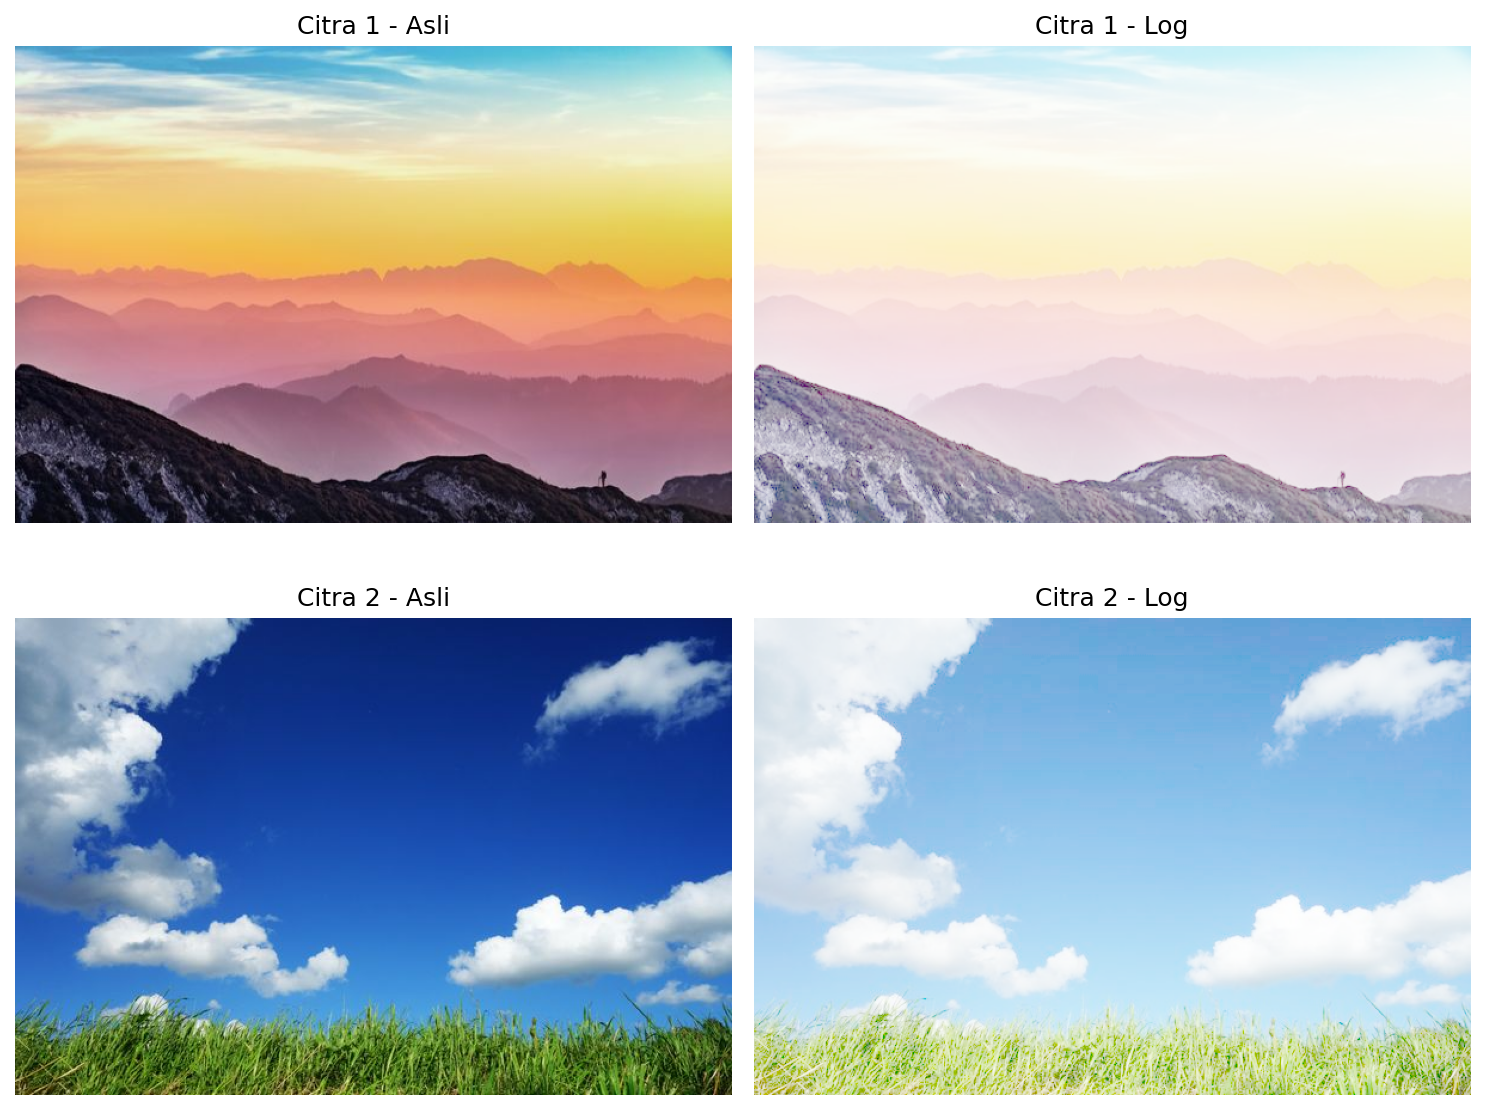
\includegraphics[width=0.85\textwidth]{fig5_log.png}
\caption{Perbandingan citra asli dan hasil transformasi logaritmik}
\label{fig:log}
\end{figure}

\textbf{Jawaban Analisis:}
\begin{enumerate}
\item Area gelap diperkuat secara signifikan karena slope log yang curam di nilai rendah.
\item Area terang dikompresi, detail pada area terang bisa berkurang.
\item Berguna untuk citra underexposed atau citra medis dengan detail samar di area gelap.
\item Risiko: mengurangi kontras pada citra yang sudah terang, membuat tampak washed out.
\end{enumerate}

% ============================================================
% 7. TRANSFORMASI GAMMA
% ============================================================
\section{Transformasi Gamma}

Transformasi gamma: $s = r^{\gamma}$ dengan normalisasi $r \in [0, 1]$. Empat nilai gamma diuji.

\begin{table}[H]
\centering
\caption{Efek nilai gamma terhadap citra}
\label{tab:gamma}
\begin{tabular}{cl}
\toprule
\textbf{Nilai $\gamma$} & \textbf{Efek terhadap Citra}\\
\midrule
0,5 & Lebih terang, kontras meningkat, detail gelap terangkat\\
1,0 & Identik dengan asli (tidak ada perubahan)\\
2,0 & Lebih gelap, kontras menurun, detail terang berkurang\\
2,5 & Jauh lebih gelap, efek shadow kuat, detail hilang\\
\bottomrule
\end{tabular}
\end{table}

\begin{figure}[H]
\centering
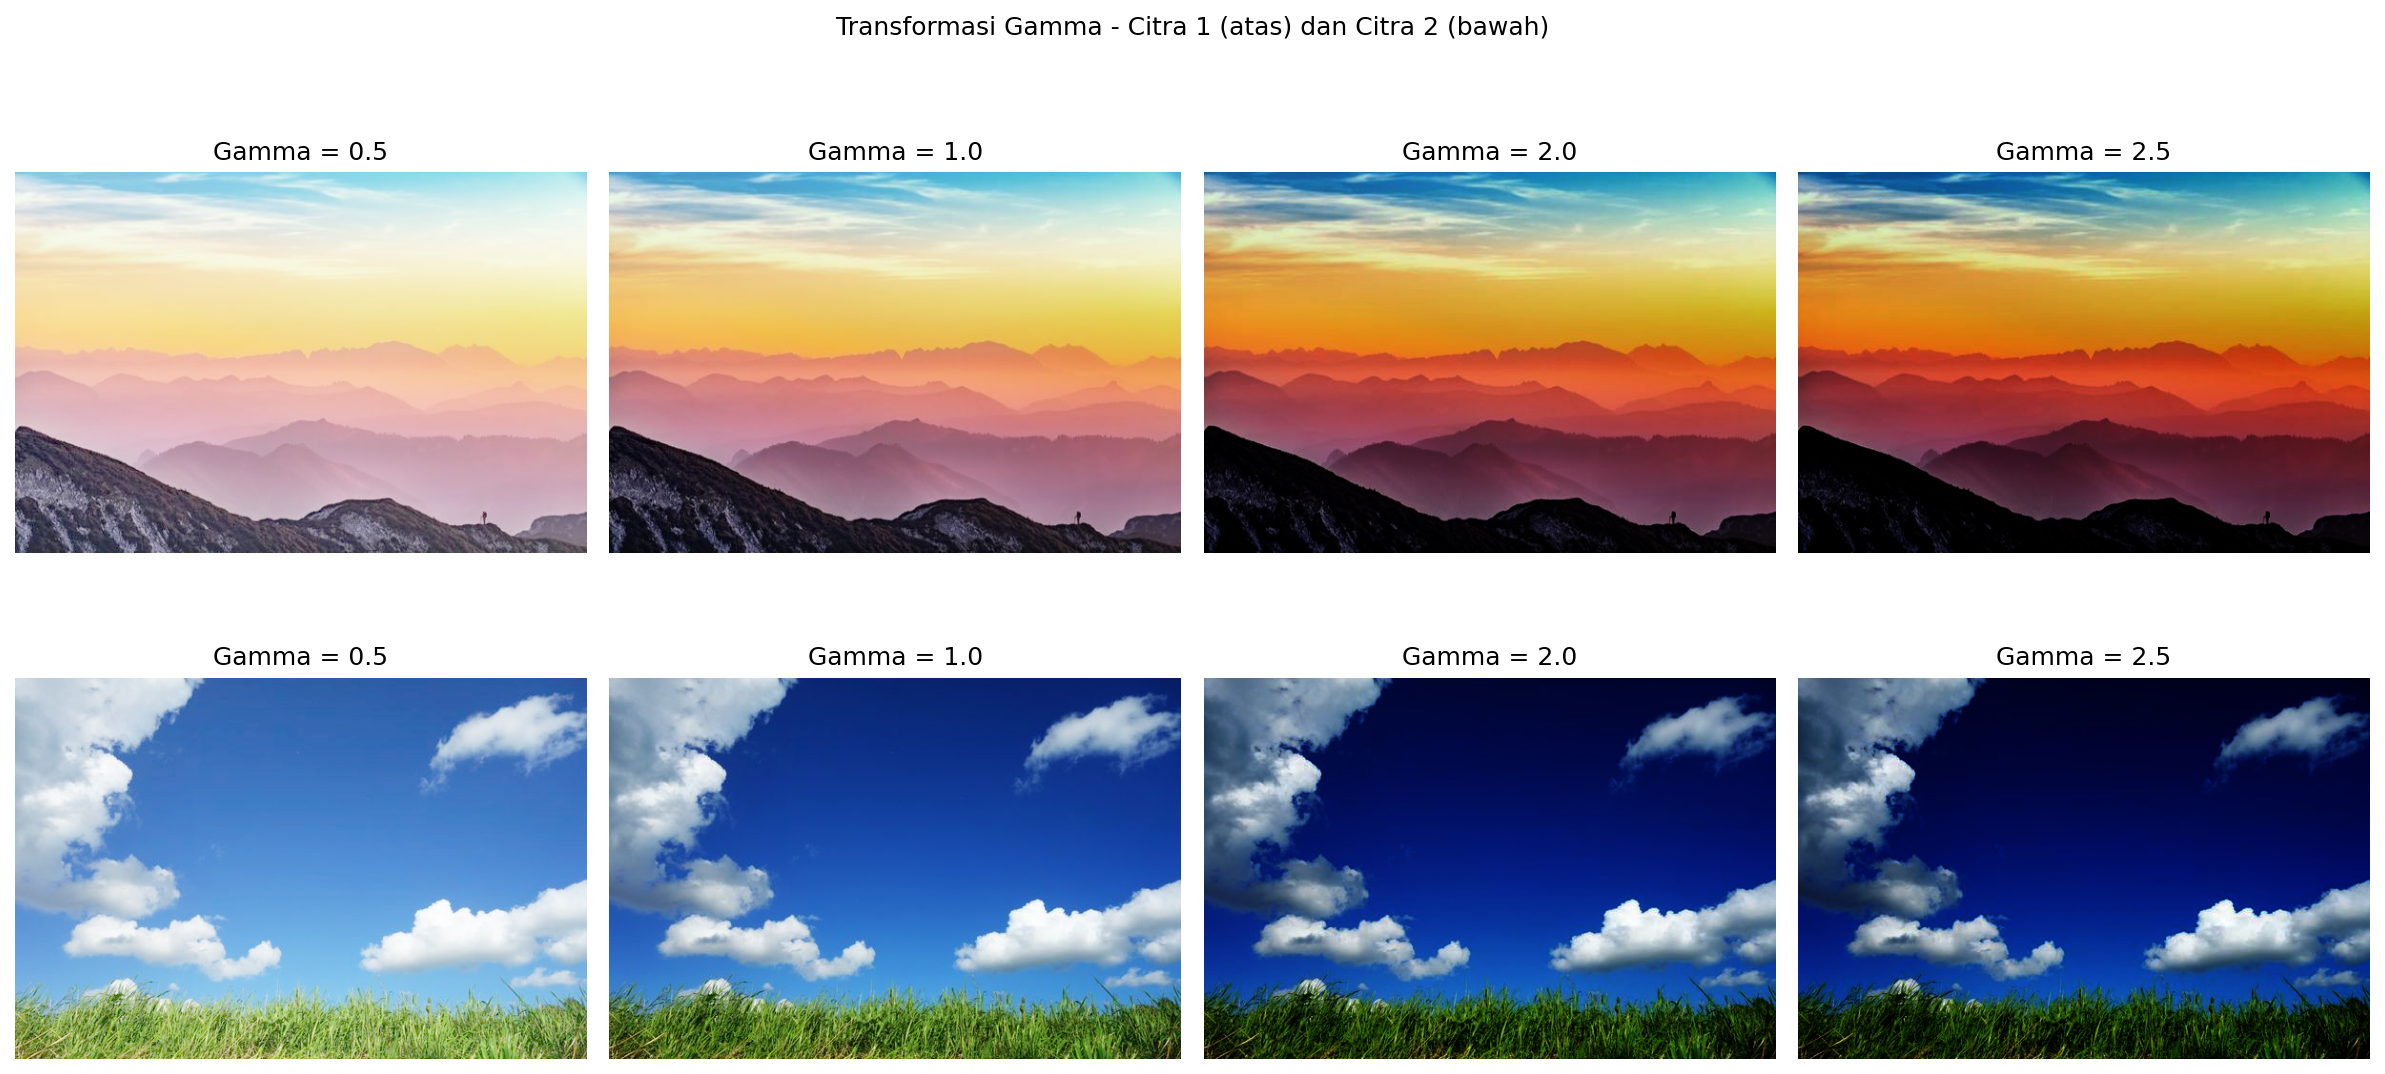
\includegraphics[width=\textwidth]{fig4_gamma.png}
\caption{Hasil transformasi gamma untuk 4 nilai $\gamma$}
\label{fig:gamma}
\end{figure}

\textbf{Jawaban Analisis:}
\begin{enumerate}
\item $\gamma < 1$: Citra lebih terang, detail gelap meningkat.
\item $\gamma = 1$: Tidak ada perubahan (referensi).
\item $\gamma > 1$: Citra lebih gelap, detail terang berkurang.
\item Koreksi pencahayaan: $\gamma < 1$ untuk underexposed, $\gamma > 1$ untuk overexposed.
\item Gamma lebih fleksibel untuk koreksi umum; log lebih spesifik untuk detail gelap.
\end{enumerate}

% ============================================================
% 8. ANALISIS HOTS DAN STUDI KASUS
% ============================================================
\section{Analisis HOTS dan Studi Kasus}

\subsection{Perbandingan Teknik}

\begin{table}[H]
\centering
\caption{Perbandingan empat teknik manipulasi citra}
\label{tab:perbandingan}
\small
\begin{tabular}{p{2.5cm}p{2.5cm}p{3.5cm}p{3.5cm}}
\toprule
\textbf{Teknik} & \textbf{Jenis Operasi} & \textbf{Efek Visual} & \textbf{Kapan Digunakan}\\
\midrule
Image Blending & Aritmatika linier & Dua citra menyatu & Menggabungkan citra, watermark\\
Image Negative & Aritmatika (255-I) & Warna terbalik & Analisis medis, efek vintage\\
Log Transform & Non-linier (log) & Gelap jadi terang & Detail area gelap, underexposed\\
Gamma Transform & Non-linier (pangkat) & Kecerahan berubah & Koreksi pencahayaan umum\\
\bottomrule
\end{tabular}
\end{table}

\subsection{Studi Kasus 1: Foto Malam Hari}

\textbf{Teknik:} Transformasi gamma ($\gamma < 1$) + Transformasi logaritmik.

\textbf{Alasan:} Gamma correction mencerahkan area gelap secara global, sementara log transform
meningkatkan detail lokal di area yang sangat gelap. Kombinasi keduanya memberikan hasil optimal.

\textbf{Risiko:} Noise pada area gelap ikut diperkuat; area terang (lampu) bisa mengalami saturasi;
hasil bisa terlihat artificial jika gamma terlalu kecil.

\subsection{Studi Kasus 3: Efek Gabungan Foto dan Tekstur Hujan}

\textbf{Teknik:} Image Blending.

\textbf{Alasan:} Blending menggabungkan dua citra dengan bobot yang bisa diatur. Foto sebagai
latar belakang ($\alpha$ besar), tekstur hujan sebagai overlay ($\beta$ kecil). Bobot menentukan
seberapa transparan efek hujan: $\beta = 0,1$ (tipis), $\beta = 0,3$ (natural), $\beta = 0,5$
(seimbang), $\beta = 0,7$ (hujan dominan).

% ============================================================
% 9. KESIMPULAN DAN REFLEKSI
% ============================================================
\section{Kesimpulan dan Refleksi Pribadi}

\subsection{Kesimpulan}

Setiap teknik manipulasi citra memiliki kelebihan dan kekurangan:
\begin{itemize}
\item \textbf{Image Blending} efektif untuk menggabungkan dua citra dengan kontrol bobot.
\item \textbf{Image Negative} membalikkan nilai pixel, berguna untuk analisis medis.
\item \textbf{Transformasi Logaritmik} sangat efektif meningkatkan detail di area gelap.
\item \textbf{Transformasi Gamma} paling fleksibel untuk koreksi pencahayaan global.
\end{itemize}

Pemilihan teknik yang tepat bergantung pada karakteristik citra dan tujuan yang ingin dicapai.
Tidak semua transformasi selalu memperbaiki kualitas citra; setiap teknik memiliki trade-off.

\subsection{Refleksi Pribadi}

\textbf{1. Teknik paling mudah dipahami:} Image negative, karena operasinya sederhana
($I = 255 - I$) dan intuitif.

\textbf{2. Teknik paling sulit dianalisis:} Image blending, karena membutuhkan eksperimen
bobot yang tepat untuk hasil yang diinginkan.

\textbf{3. Perbedaan log dan gamma:} Logaritmik lebih agresif di area gelap; gamma lebih
fleksibel untuk koreksi keseluruhan dengan kontrol nilai $\gamma$.

\textbf{4. Hal baru yang dipahami:} Nilai pixel bukan sekadar angka, melainkan representasi
intensitas yang dapat dimanipulasi secara matematis. Setiap transformasi memiliki trade-off.

\textbf{5. Teknik pertama untuk aplikasi:} Transformasi gamma karena fleksibilitasnya tinggi,
bisa mencerahkan ($\gamma < 1$) maupun menggelapkan ($\gamma > 1$) citra.

\end{document}
